%------------------------------------------------------------------------
% Chapter:  Appendix Installation
%------------------------------------------------------------------------

\chapter{Installation \label{app-install}}

In this section we will describe the installation process
for the \Discus program package. 
The current version of the
software can be downloaded from the \Discus homepage at \\
\url{
https://github.com/tproffen/DiffuseCode/}. \\
Refer to the section corresponding
to your operating system for installation information.

At the github release site you will find installation guides for
\Discus for Unix, MacOS and Cygwin.  The Windows installation is performed
via a self extracting installer.

%------------------------------------------------------------------------
\section{Windows \label{appa-bwin}}

The Windows version of the \Discus package is distributed as a
self-extracting installer. This makes the installation very easy.
Simply download the file {\it Diffuse-X.X.X-win64-YYMMDD.exe} or
if necessary {\it Diffuse-X.X.X-win32-YYMMDD.exe}. Here YYMMDD
specifies the date of the distribution and. X.X.X stands for the 
version number. Make sure you download the
most recent one.  Run the installer by double clicking on the
corresponding file icon. You will first receive a Windows security
alert, % (Fig. \ref{fig-winstall}), 
because the installer is not digitally 
signed by us. Once we get around to figure out how, this warning will go 
away. For now, just click on {\it Run}. This will start the installation 
process itself and the installation dialog will show up. %n in Fig. \ref{fig-winstall} will appear. 
Follow the instructions on the screen and that is all, you are ready to use
any of the programs that are part of the \Discus package. Look
in the {\it START - Programs} menu for links to the programs as well
as the documentation.

As you may noticed, we have changed the way the installer is build. For 
that reason, you need to \textbf{uninstall any \Discus version prior to
2010 before proceeding with the installation.} The current installer 
works fine on \textit{Windows XP, Windows Vista Windows7} and 
\textit{Windows 10}. 

%------------------------------------------------------------------------
\subsection{\Discus and CYGWIN}

The \Discus package for Windows is developed using the \textit{CYGWIN} 
package \\ \url{http://www.cygwin.com} \\
which provides a UNIX like environment 
for Windows. We recommend installing the \textit{CYGWIN} 32bit or 64 bit 
package to be used 
with the \Discus package, although this is not required. One side effect of 
the use of \textit{CYGWIN} is that one needs to specify UNIX style paths. 
Also you might see that for example drive C: is  referred to as 
{\tt /cygdrive/c/}.

Another side effect is the file format for all ASCII or text files like
macros, cell files, diffraction pattern output etc. Unfortunately UNIX and
Windows use a different encoding to signal the end of a line for such file types.
Since we use \textit{cygwin}, the file format is UNIX style. As a consequence,
the Windows \textit{Editor} usually found under \textit{All programs} 
in the \textit{Accessories} section cannot handle such
file types. Please use a more advanced text editor like \textit{Notepad+} 
or \textit{WordPad} instead to edit these files.
If you installed \textit{CYGWIN}, you can use the programs \textit{unix2dos}
and \textit{dos2unix} to convert file formats.

%\begin{figure}[!bt]
%   \centering
%   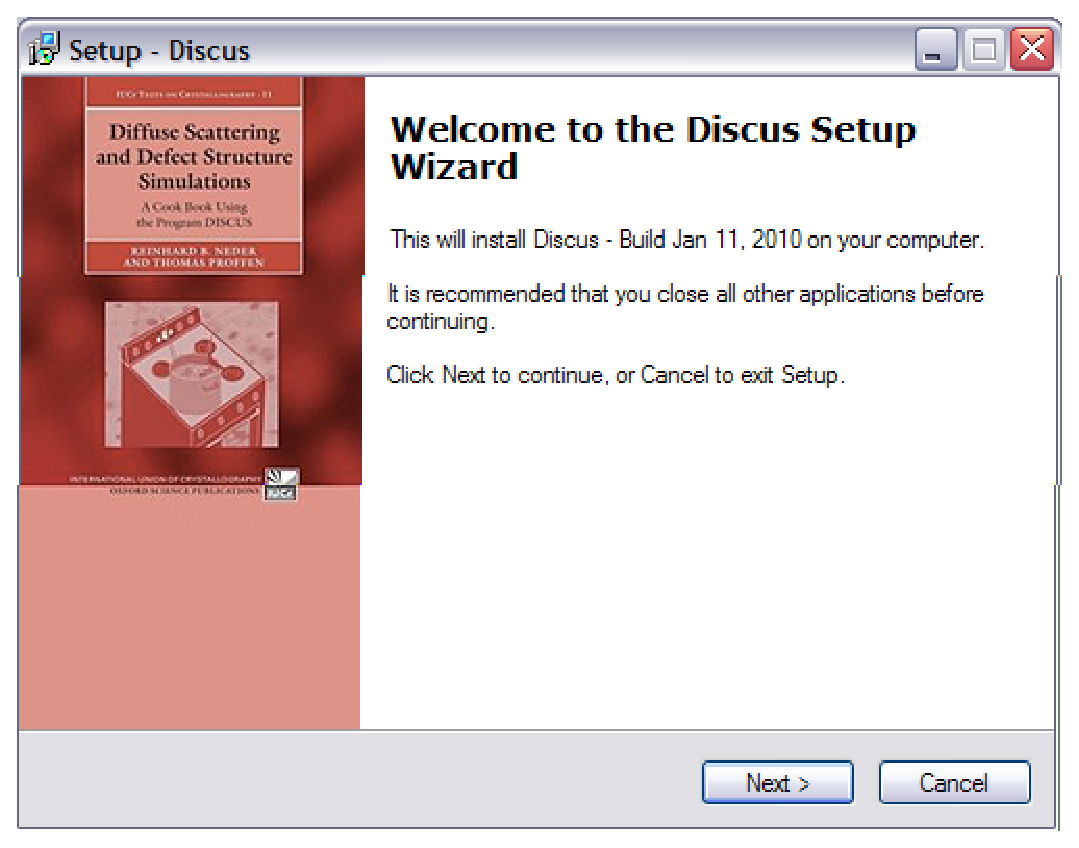
\includegraphics[width=3.0in]{winstall.eps}
%   \hspace{5mm}
%   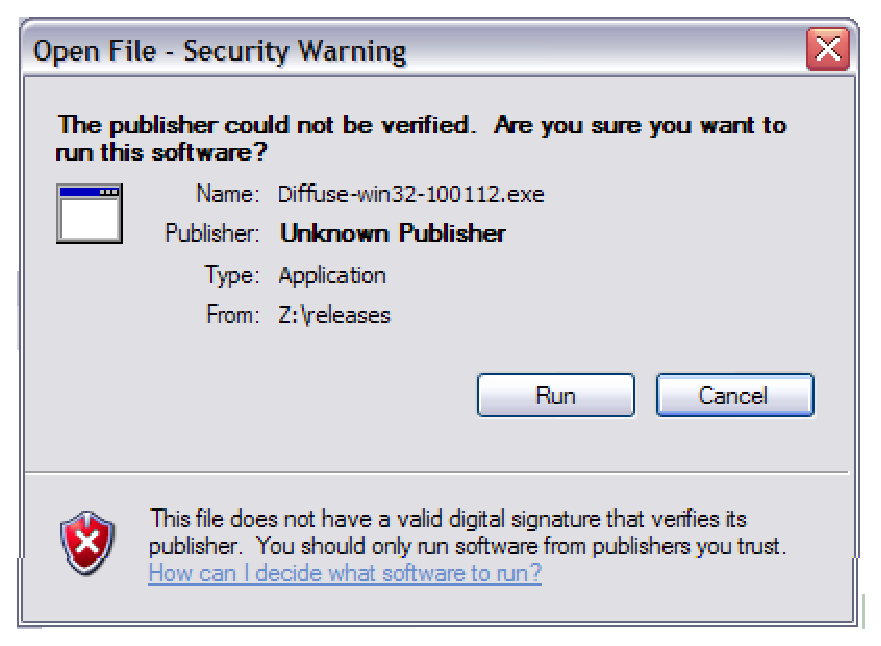
\includegraphics[width=1.7in]{wwarn.eps}
%   \caption{Left: Windows installer for \Discus package.
%            Right: Windows security warning.}
%   \label{fig-winstall}
%\end{figure}

%------------------------------------------------------------------------
\section{Mac OSX\label{appa-bmac}}

The Mac OSX version of the \Discus package is distributed as a binary
installer as well. Simply download the the file {\it Diffuse-mac-YYMMDD.exe}. 
Again YYMMDD specifies the date of the distribution. Make sure you 
download the most recent one. Once the download is finished, run the 
installer by double clicking on the corresponding file icon. You will see 
an installation screen. Follow
%a screen similar to the one shown in Fig. \ref{fig-minstall}. Follow 
the instructions. The programs will be installed in {\tt /Applications/discus}.
%
%\begin{figure}[!tb]
%   \centering
%   \includegraphics[width=3.0in]{minstall.eps}
%   \caption{Mac installer for \Discus package}
%   \label{fig-minstall}
%\end{figure}

%------------------------------------------------------------------------
\section{Unix / Linux \label{appa-bunix}}

For Unix or Linux operating systems, the \Discus package is
distributed as source code and needs to be compiled before the
programs can be used. You might also check the \Discus homepage for
available binary distributions for Linux which might be available
in the near future. 
Refer to the separate file {\tt INSTALL\_DISCUS.pdf} 
or {\tt AAA\_INSTALL\_DISCUS.pdf} for details.

To build the programs from the source, you will 
need a FORTRAN and a C compiler. We use {\tt gcc} and {\tt gfortran}
which are freely available at\\ 
\url{http://directory.fsf.org/project/gcc/}. \\
While {\tt gcc} is installed on most Linux systems, {\tt gfortran} might
need to be installed separately.

First copy or download the file {\it DIFFUSE\_CODE\_YYYY\_MMDD.tar.gz} or
from the github release pages the link to {\it vX.X.X.tar.gz}. Next
unpack the archive using the command

\begin{MacVerbatim}
    tar -xvf DIFFUSE_CODE_YYYY_MMDD.tar.gz
\end{MacVerbatim}

This will create a directory {\it DiffuseCode}, containing the
distribution. Within this directory there are separate directories
for each of the different programs as well as a directory {\it lib\_f90}
which contains command language related routines common to all
programs. Build a a new Directory called {\it DiffuseBuild} next to the
source code directory. Go to this build directory and run ccmake to 
install the program:

Finally some environment variables need to be defined. Each program
looks for a variable corresponding to its name. For example \Discus 
will use a variable {\tt DISCUS} and so on. The definition of 
the variables can be done e.g. in the {\it .login} or {\it .cshrc} file 
using the command {\it setenv DISCUS /path/to/discus} for 
the {\it csh} of {\it set DISCUS=/path/to/discus; export DISCUS} if 
you are using the 
Bourne shell. If this path is also included in your search path you can
start the program simply by entering {\it discus}. Similarly, the
other programs are started by entering their respective names.

%------------------------------------------------------------------------

%\section{Please register}

%Please register yourself as a user of one or more programs of the
%\Discus program package. In the top directory of the
%distribution you will find the file {\tt REGISTER}. Please fill in
%the corresponding information and send the file via email to {\it
%tproffen@lanl.gov}. We also recommend that you subscribe to the 
%{\tt discus-announce@lists.sourceforge.net} mailing list to stay
%informed of the release of new versions of the \Discus package. 
%Details can be found on the \Discus homepage at 
%\url{http://discus.sourceforge.net}.

%------------------------------------------------------------------------
